\documentclass[tikz,border=3mm]{standalone}
\usetikzlibrary{shapes.geometric, arrows.meta}

\begin{document}
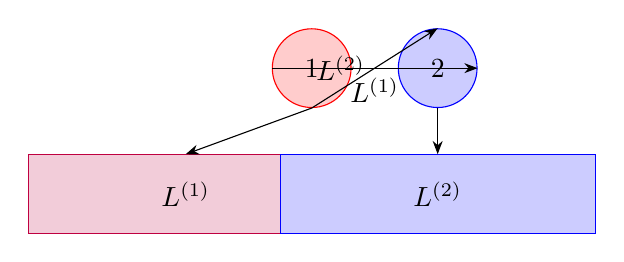
\begin{tikzpicture}[scale=0.8]

% Define colors
\tikzset{
    red/.style={draw=red, fill=red!20},
    blue/.style={draw=blue, fill=blue!20},
    purple/.style={draw=purple, fill=purple!20}
}

% Nodes for q-Boson model
\node[red, circle, minimum size=1cm] (b1) at (0,0) {1};
\node[blue, circle, minimum size=1cm] (b2) at (2,0) {2};

% Lines connecting q-Boson nodes
\draw[-Stealth] (b1.south) -- node[midway, below] {$\bm{L}^{(1)}$} (b2.north);
\draw[-Stealth] (b1.west) -- node[midway, left] {$\bm{L}^{(2)}$} (b2.east);

% Ensembles
\node[purple, rectangle, minimum width=4cm, minimum height=1cm, align=center] (l1) at (-2,-2) {\(\bm{L}^{(1)}\)};
\node[blue, rectangle, minimum width=4cm, minimum height=1cm, align=center] (l2) at (2,-2) {\(\bm{L}^{(2)}\)};

% Connect q-Boson model to ensembles
\draw[-Stealth] (b1.south) -- (l1.north);
\draw[-Stealth] (b2.south) -- (l2.north);

\end{tikzpicture}
\end{document}